\chapter{Profiling}\label{sec:profiling}

We include here results from profiling to identify where to put the effort to further optimize the code. The diagrams shown below have been constructed with {\tt gprof2dot.py}\footnote{\url{https://github.com/jrfonseca/gprof2dot}}.

\begin{figure}[H]
  \centering
  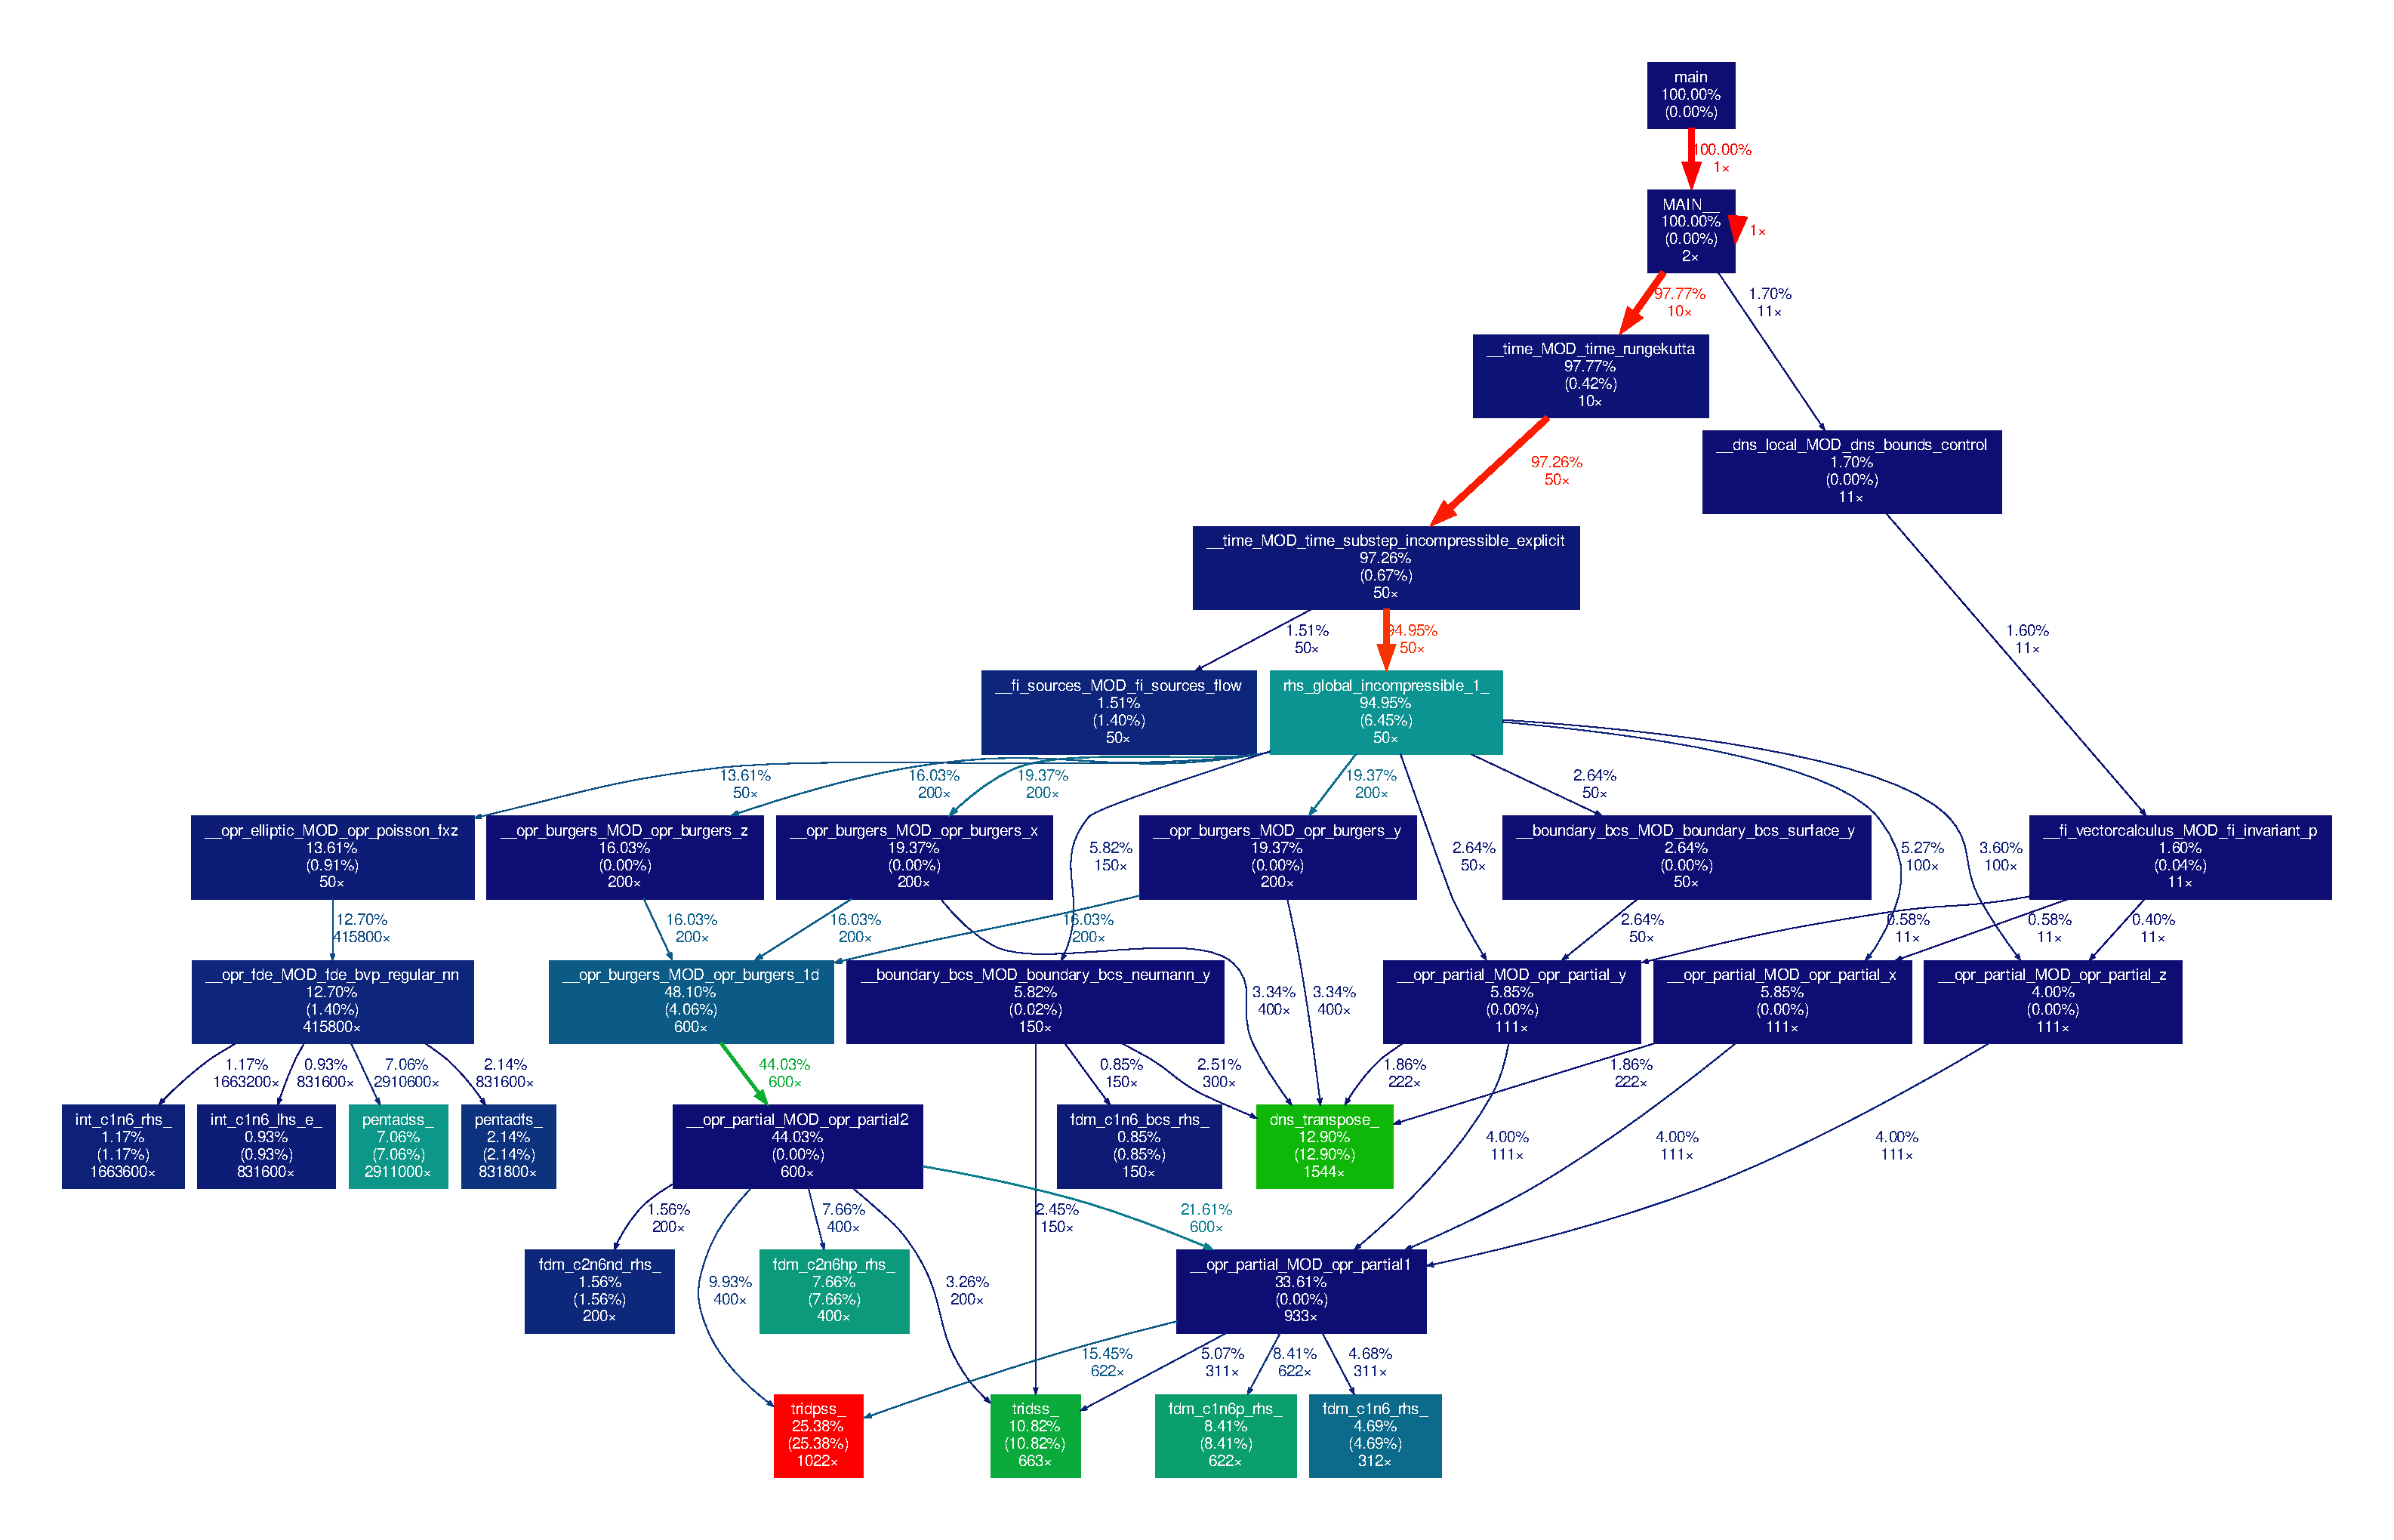
\includegraphics[clip,width=\textwidth]{figs/profiling.pdf}
  \caption{Profiling diagram of {\tt examples/Case44} running 10 iterations in serial mode. Profiling data obtained from {\tt gfortran -pg} and processed with {\tt gprof}, running the command {\tt gprof path/to/your/executable | gprof2dot --color-nodes-by-selftime | dot -Tpdf -o output.pdf}.}
\end{figure}

\begin{figure}[H]
  \centering
  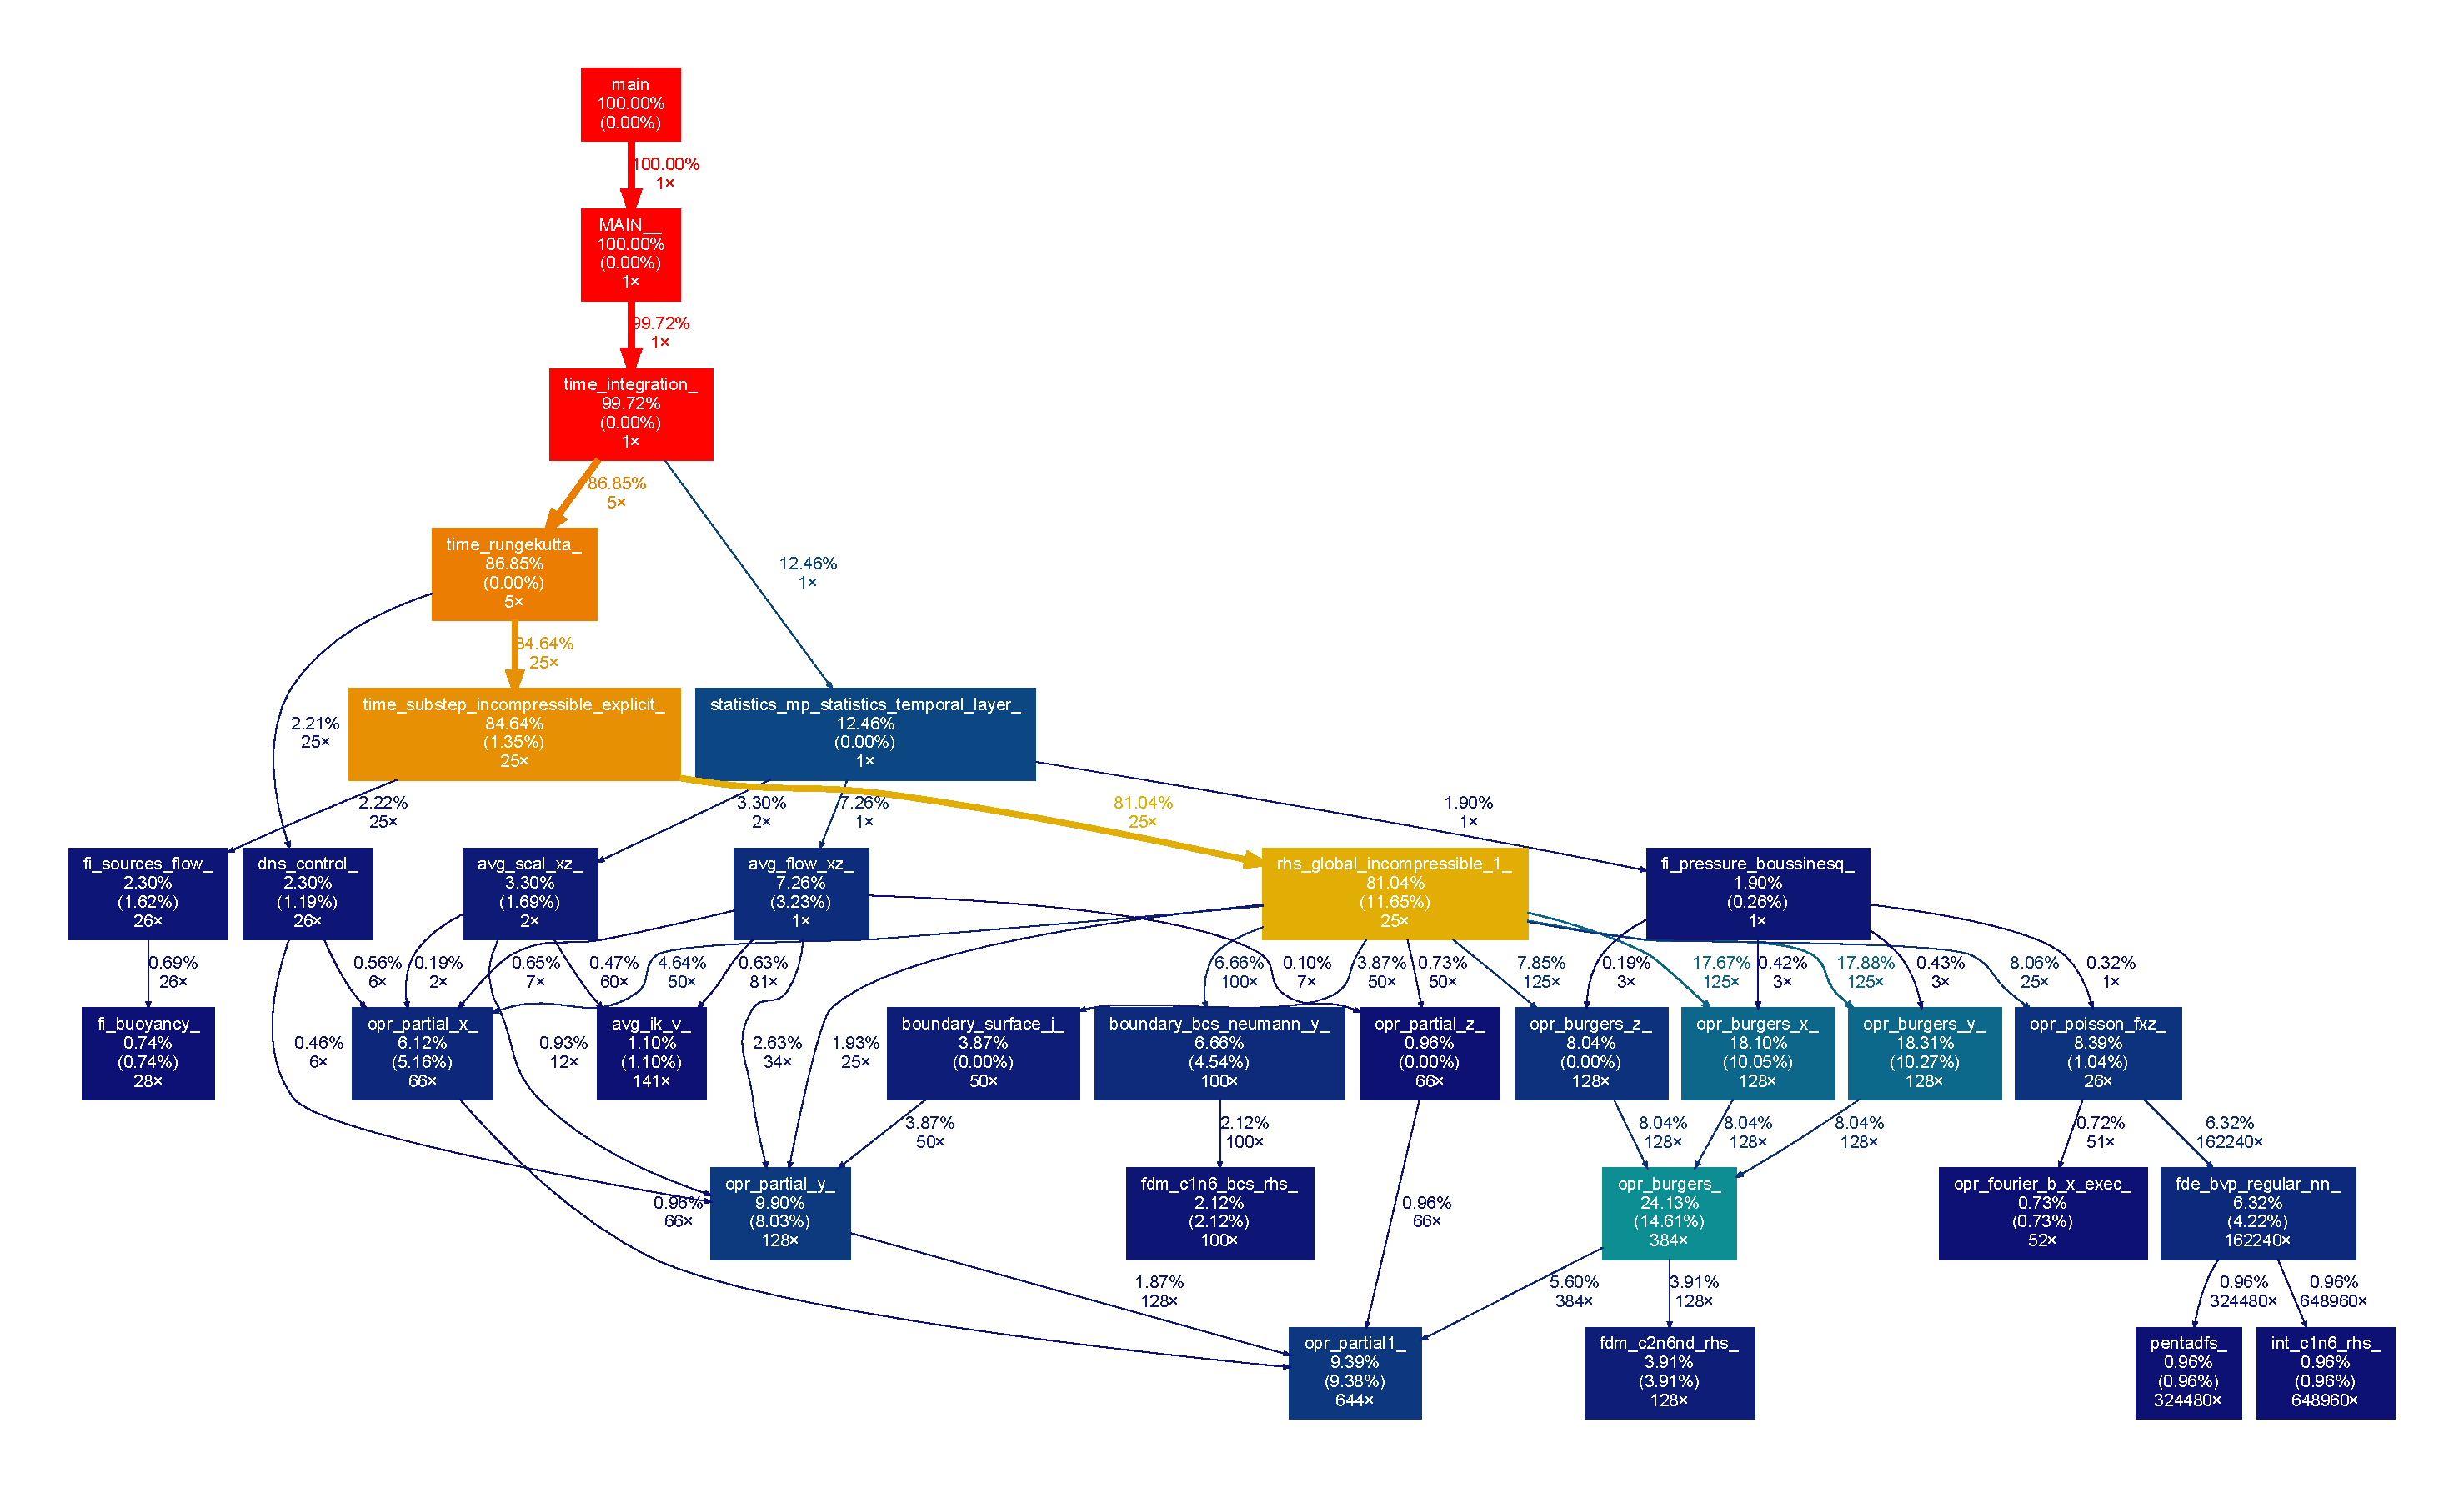
\includegraphics[clip,width=\textwidth]{figs/profiling2.pdf}
  \caption{Profiling diagram of modified {\tt examples/Case44} (768 cube) running 25 iterations in parallel mode with 48 tasks (1 node on juwels).}
\end{figure}

